\documentclass{jarticle}
\usepackage[dvipdfmx]{graphicx}
\usepackage{here}
\usepackage{amsmath}
\usepackage{latexsym}
\usepackage{multirow}
\usepackage{textcomp}
\usepackage{url}
\usepackage{array}    % 列の設定
\usepackage{caption}
\usepackage{booktabs}
\usepackage[utf8]{inputenc}
\newcommand{\ita}{\textit}
\newcommand{\ko}{\rm{k$\Omega$}}
\newcommand{\om}{\rm$\Omega$}
\newcommand{\nf}{\rm{nF}}
\title{}
\date{}
\begin{document}\maketitle




\section{実験内容}
\subsection{実験１}
まず、RC 直列回路に対して 1\,V の直流電圧源を $t = 0$ で印加したときの
コンデンサ電圧 $V_c$ の過渡応答を LTspice を用いて観測した。

過渡現象が明確に観察できるように、抵抗およびコンデンサの値として


\[
R = 10\,\text{k}\Omega,\qquad C = 10\,\mu\text{F}
\]
を選んだ。
電圧源にはPULSE関数を用い、パラメータを以下のように設定した。
\begin{table}[H]
    \centering
    \caption{PLUSE関数のパラメータ}
    \begin{tabular}{cc}
    \toprule
    パラメータ & その値 \\
    \midrule
    初期電圧 & 0 V \\
    パルス振幅 & 1 V \\
    遅延時間 & 0 s\\
    立ち上がり時間 & 1 ns \\
    立ち下り時間 & 1 ns \\
    パルス幅 & 10 s\\
    パルス周期 & 15 s\\
    \bottomrule
    \end{tabular}
\end{table}

そして、$V_c$ の時間表現を求め、観測値と比較検討を行った。
以下に実験に用いた回路図を示す。
\begin{figure}[H]
    \centering
    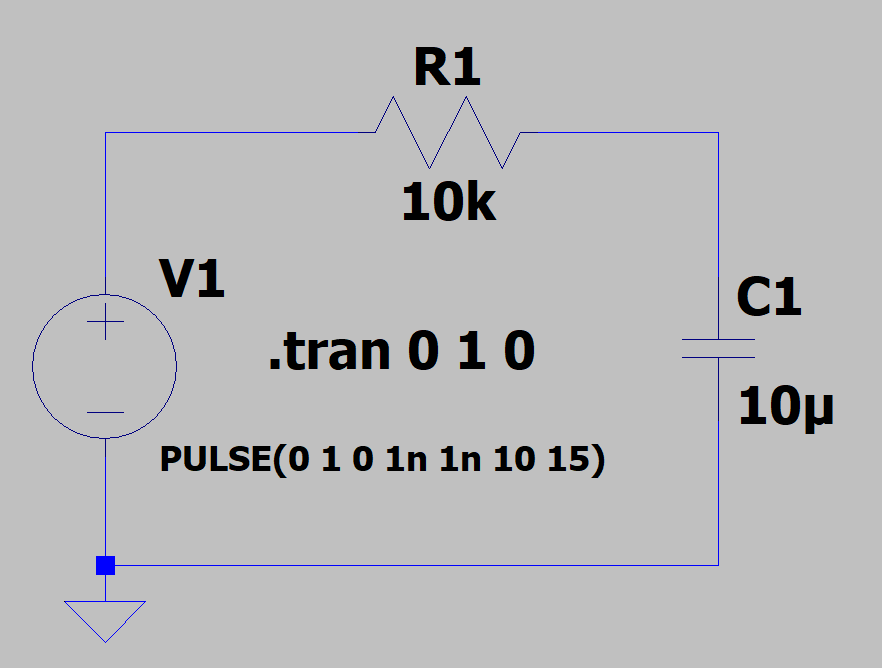
\includegraphics[width=0.7\linewidth]{sim1.png}
    \caption{RC直列回路(直流電圧源の場合)}
\end{figure}

\subsection{実験２}

直流入力に対するRC回路の過渡応答において、時定数 $T = RC$ に対し，コンデンサ電圧が定常状態に達するまでの時間を評価した。

前節と同様の回路および条件を用い，コンデンサ電圧 $V_c$ の波形から，電圧が最終値に十分近づいたとみなせる時刻を目視により見積もり，
その時刻を $t = nRC$ として $n$ の値を求めた。

\subsection{実験３}

RC直列回路の電圧源を交流電圧源に変更し、入力電圧を
$V(t)=\sin(\omega t)$とした。周波数 $f$ は回路の応答が適切に観測できるように10 Hzとした。
この条件で過渡解析を行い，コンデンサ電圧 $V_c$ の波形を観測した。

さらに，前節で求めた $t = nRC$ を観測開始時刻とし，過渡成分が十分に減衰し，波形が定常状態となっていることを確認した．
以下に実験に用いた回路図を示す。
\begin{figure}[H]
    \centering
    \includegraphics[width=0.7\linewidth]{draft2.png}
    \caption{RC直列回路の応答(交流電圧源の場合)}
\end{figure}

\subsection{実験４}

前節と同様の条件のもとで，回路に流れる電流 $I$ の定常状態における波形を観測した。

また，同一条件における電流 $I$ をフェーザ法により求め，その結果を位相を含めた時間領域の式に変換した。

さらに，得られた理論値とシミュレーションによる観測値との比較を行った。

\section{結果}
\subsection{実験１}
シミュレーションにより得た、入力電圧と出力電圧の波形を以下に示す。
\begin{figure}[H]
    \centering
    \includegraphics[scale=0.25]{Draft1.png}
    \caption{RC直列回路の応答}
\end{figure}

\subsection{実験２}
図3の入力電圧を取り除き、定常状態あたりを拡大したものを以下に示す。
\begin{figure}[H]
    \centering
    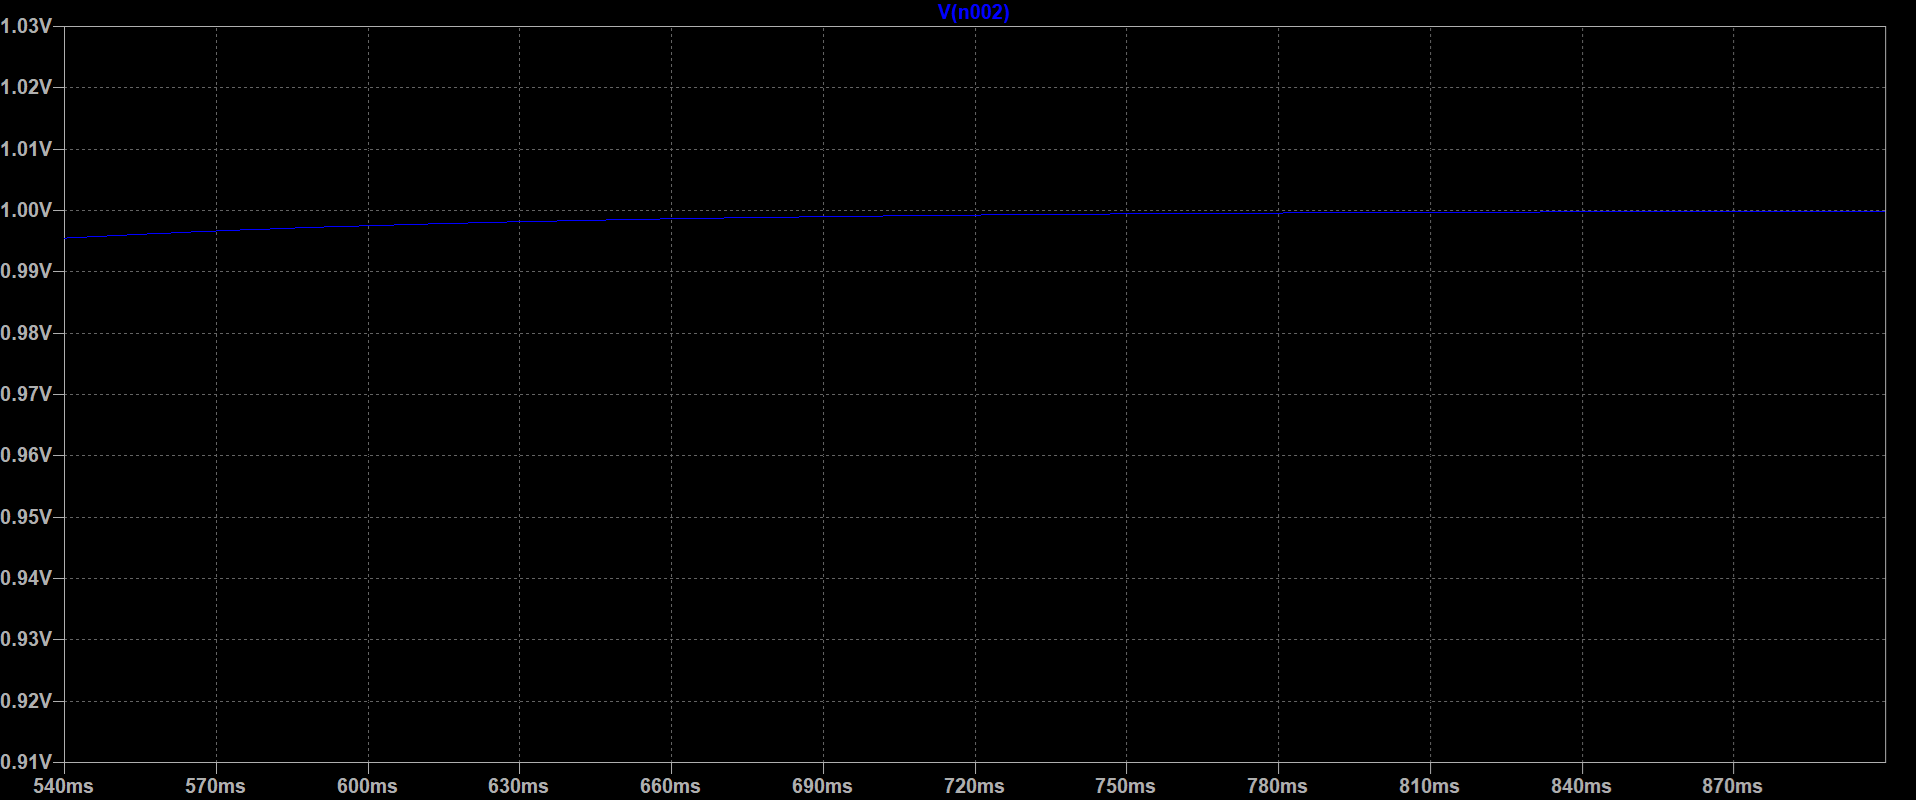
\includegraphics[scale=0.25]{sim1-2.png}
    \caption{図２の拡大図}
\end{figure}
図4よりおおよそ830$\,\mathrm{ms}$
で定常解に達しているあることがをわかる。
時定数は$T = RC = 10\,\text{k}\Omega \times 10\,\mu\text{F} = 100\,\mathrm{ms}  $
であるから、$t = 830\,\mathrm{ms} $とすると、$t = nRC$ としたときの $n$ の値は
\begin{equation*}
    n = \frac{t}{RC} = \frac{t}{T} = \frac{830}{100} = 8.3
\end{equation*}
である。

\subsection{実験３}
シミュレーションにより得た入力電圧と出力電圧の過渡解の波形を以下に示す。
\begin{figure}[H]
    \centering
    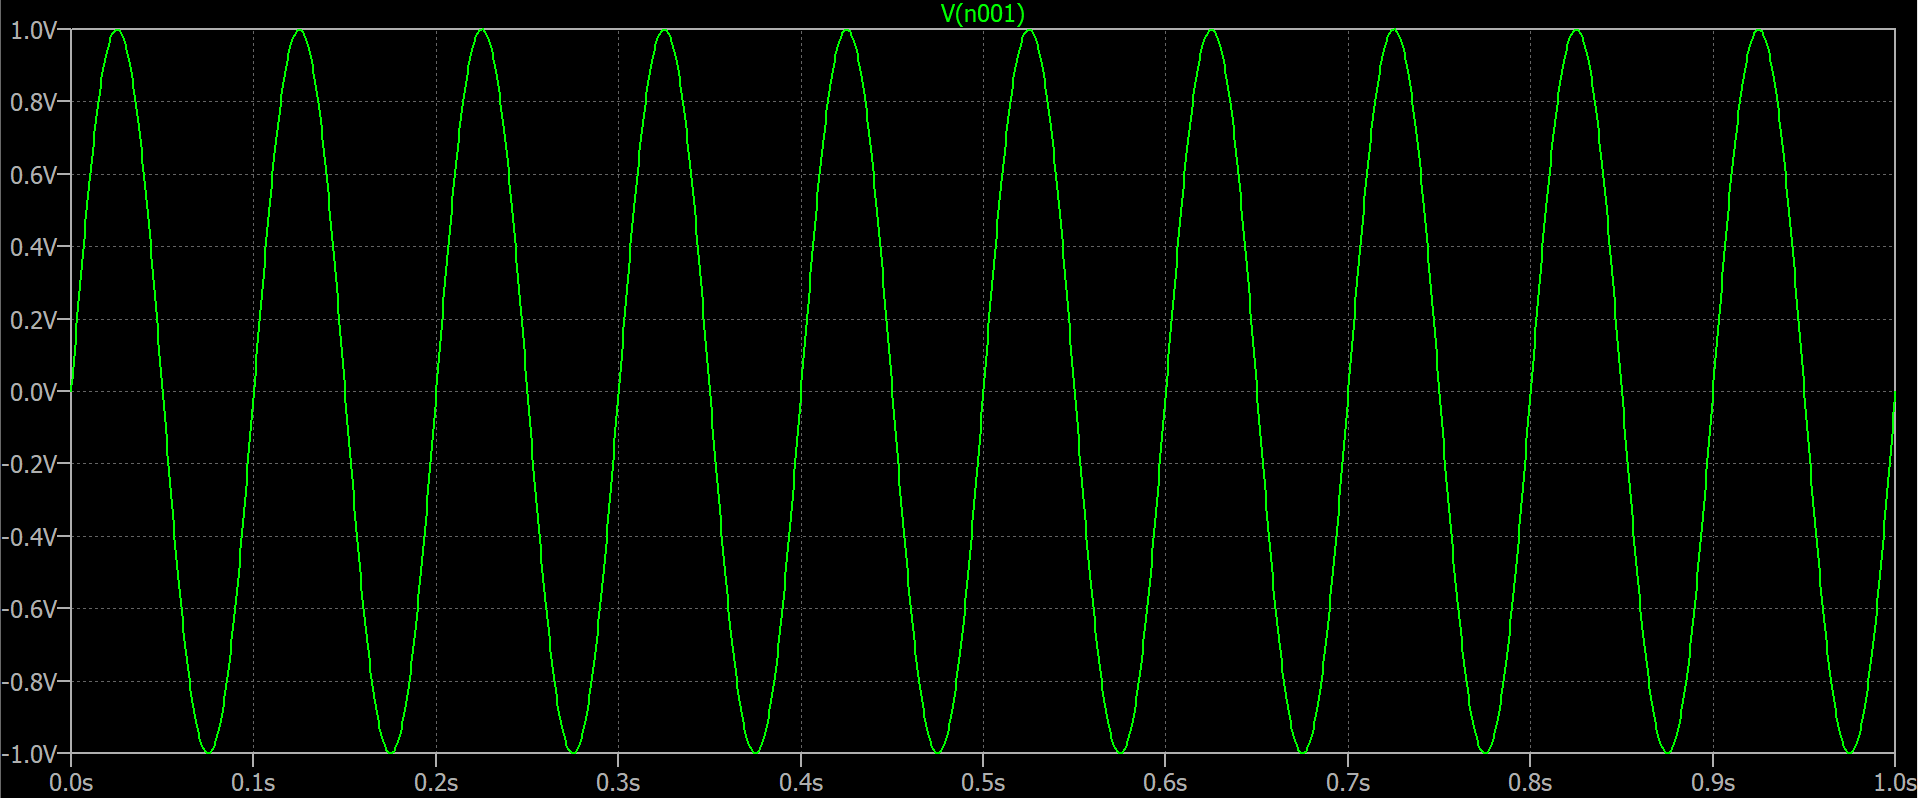
\includegraphics[scale=0.25]{sim1-7.png}
    \caption{入力電圧}
\end{figure}
\begin{figure}[H]
    \centering
    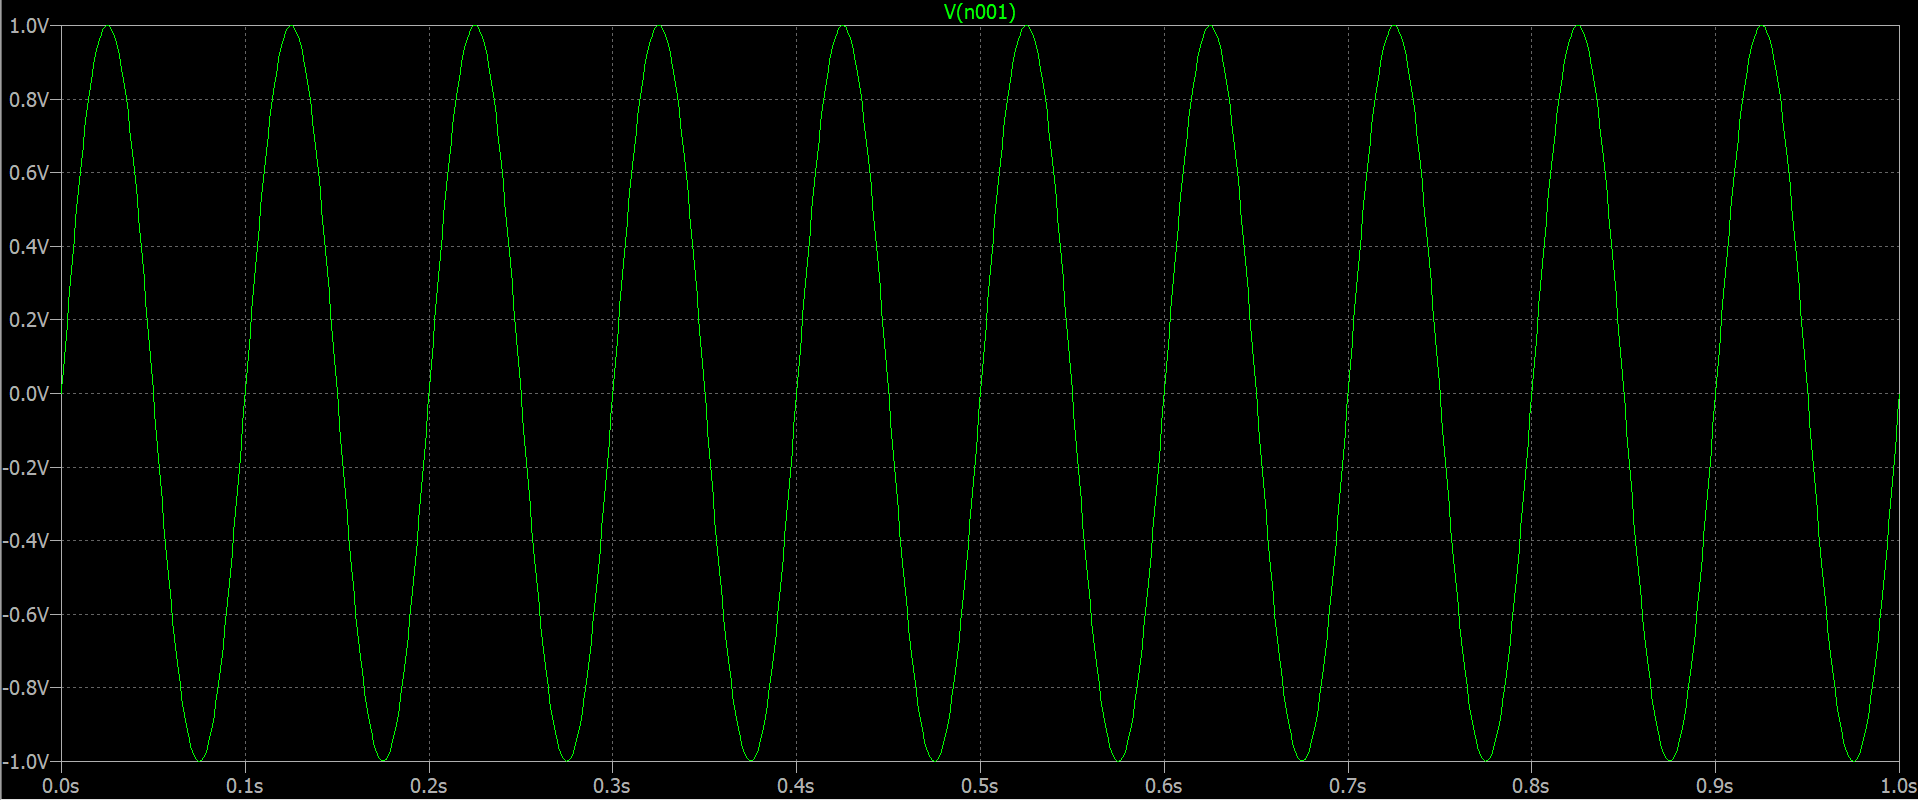
\includegraphics[scale=0.25]{sim1-5.png}
    \caption{過渡解の波形}
\end{figure}
次に$t = 830\,\mathrm{ms} $を観察開始時刻とした時の出力電圧の波形を以下に示す。
\begin{figure}[H]
    \centering
    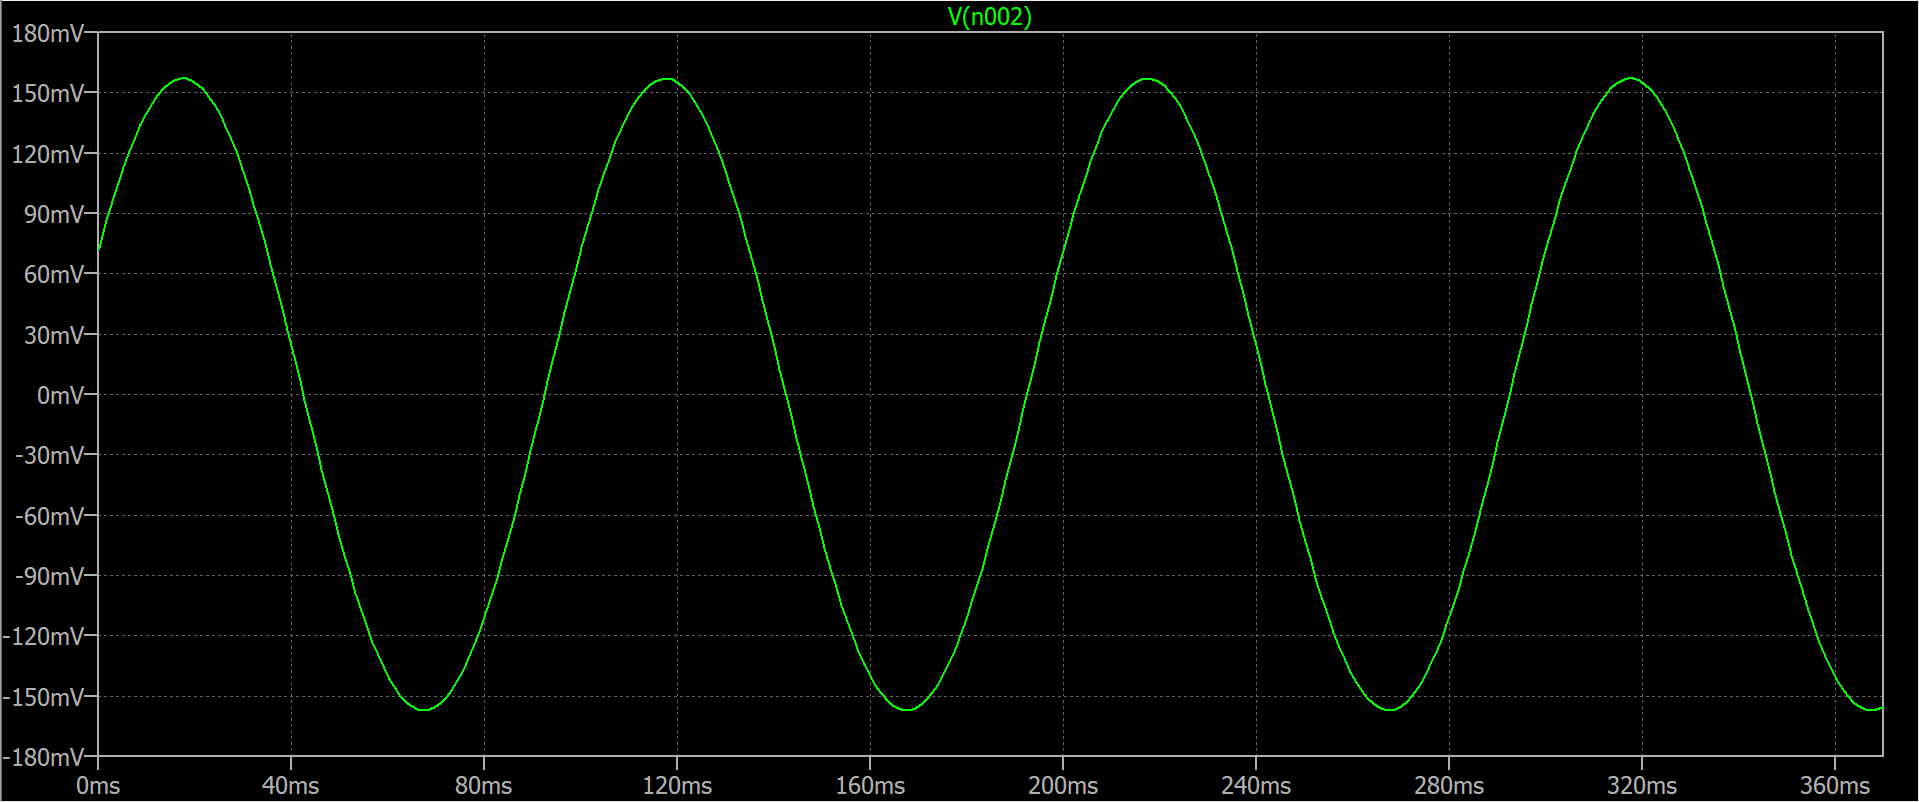
\includegraphics[scale=0.25]{sim1-8.png}
    \caption{定常解の波形}
\end{figure}

\subsection{実験４}
定常状態での電流の波形を以下に示す。
\begin{figure}[H]
    \centering
    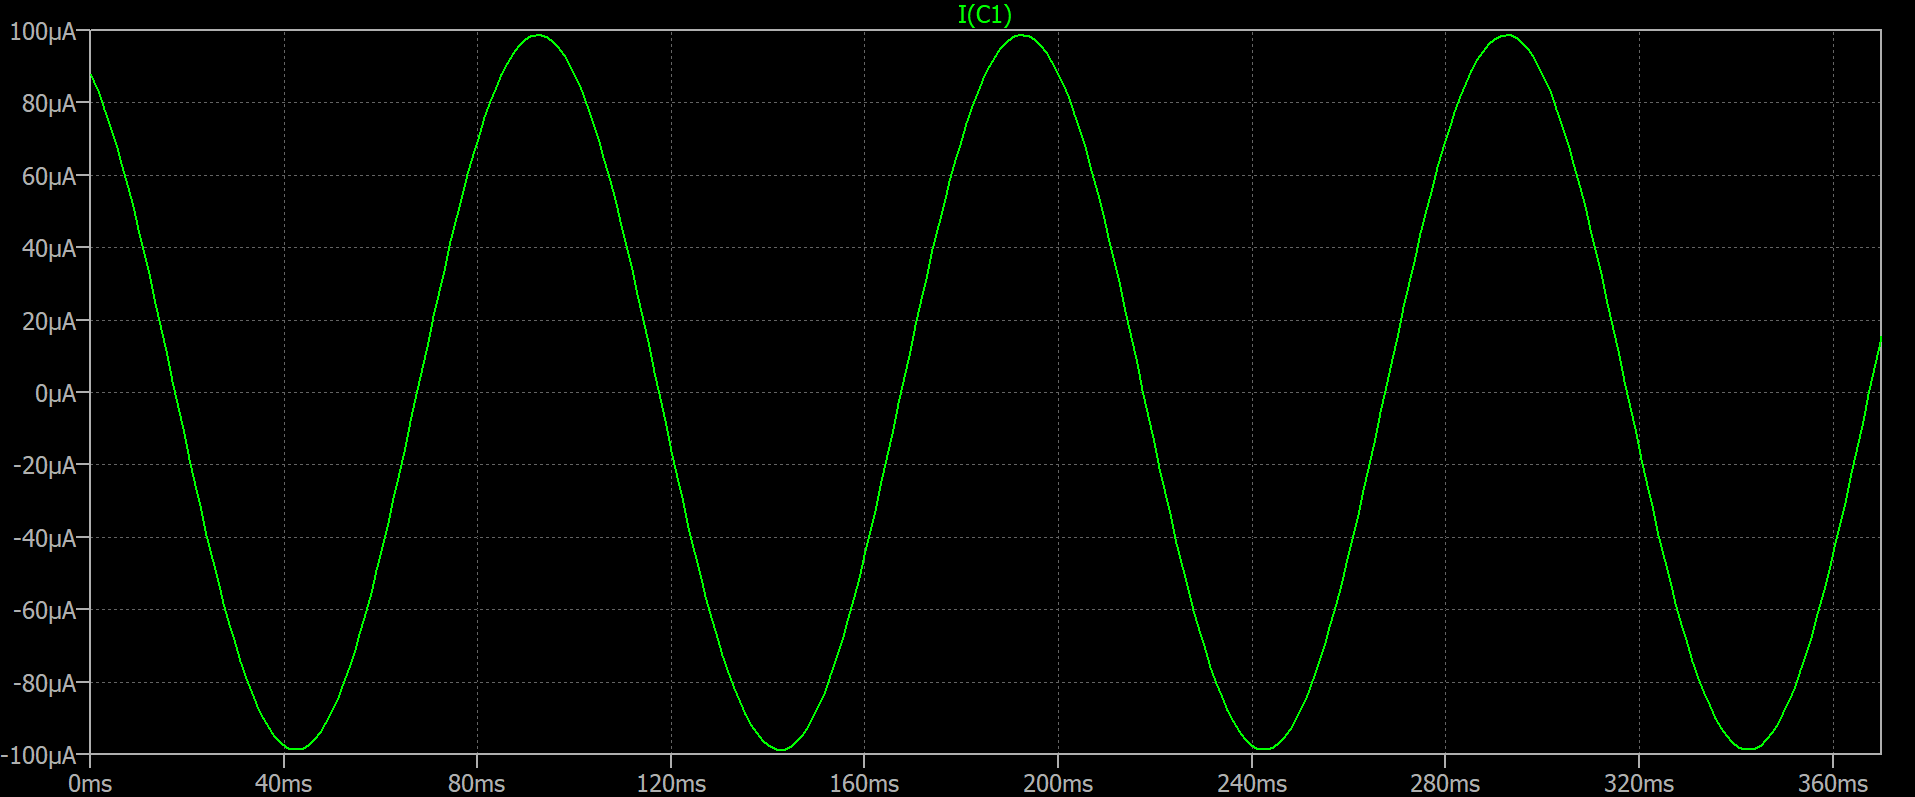
\includegraphics[scale=0.25]{sim1-9.png}
    \caption{定常解の電流の波形}
\end{figure}
次に電流$I$をフェーザ法で求める。
まず，入力電圧のフェーザ表示を
\[
V = 1 \angle 0
\]
とする。
RC直列回路のインピーダンスは
\[
Z = R + \frac{1}{j\omega C}
\]
である。
したがって，電流のフェーザ$I$は
\[
I = \frac{V}{Z} = \frac{1}{R + \frac{1}{j\omega C}}
\]

となる。
ここで分母を整理すると，
\[
Z = R - j\frac{1}{\omega C}
\]

であるから，
\[
|Z| = \sqrt{R^2 + \left(\frac{1}{\omega C}\right)^2}
\]

また，位相は
\[
\angle Z = -\tan^{-1}\left(\frac{1}{\omega RC}\right)
\]

となる。
よって電流のフェーザは
\[
I = \frac{1}{\sqrt{R^2 + \left(\frac{1}{\omega C}\right)^2}}
\angle \tan^{-1}\left(\frac{1}{\omega RC}\right)
\]

となる。
これを時間領域に戻すと，
\begin{equation}
I(t)=\frac{1}{\sqrt{R^2 + \left(\frac{1}{\omega C}\right)^2}}
\sin\left(\omega t + \tan^{-1}\left(\frac{1}{\omega RC}\right)\right)
\end{equation}

となる。

\section{考察}
\subsection{実験１}

RC直列回路において、時刻$t=0$で1\,Vのステップ電圧を印加した場合のコンデンサ電圧$V_c(t)$を求める。

回路において，キルヒホッフの法則より
\[
V(t) = V_R(t) + V_c(t)
\]
が成り立つ。
ここで，入力電圧はステップ関数として
\[
V(t) = 1 \quad (t \geq 0)
\]
とする。
また，抵抗の電圧は
\[
V_R(t) = R i(t)
\]
であり，コンデンサ電流は
\[
i(t) = C \frac{dV_c(t)}{dt}
\]
である。
したがって，
\[
V_R(t) = RC \frac{dV_c(t)}{dt}
\]
となる。
これを回路方程式に代入すると，
\[
1 = RC \frac{dV_c(t)}{dt} + V_c(t)
\]
を得る。
この微分方程式をラプラス変換すると，
\[
\frac{1}{s} = RC \left(sV_c(s) - V_c(0)\right) + V_c(s)
\]

初期条件 $V_c(0)=0$ を用いると，
\[
\frac{1}{s} = RC \, s V_c(s) + V_c(s)
\]

\[
V_c(s)\left(RC s + 1\right) = \frac{1}{s}
\]

\[
V_c(s) = \frac{1}{s(RC s + 1)}
\]

部分分数分解を行うと，
\[
V_c(s) = \frac{1}{s} - \frac{1}{s + \frac{1}{RC}}
\]

これを逆ラプラス変換すると，
\[
V_c(t) = 1 - e^{-t/RC}
\]

となる。ここに$R = 10\,\text{k}\Omega, C = 10\,\mu\text{F}$を代入すると
\begin{equation}
V_c(t) = 1 - e^{-10t}    
\end{equation}

(2)式を用いて，各時刻におけるコンデンサ電圧の理論値を算出した。
また、同時にLTspiceによるシミュレーション値を取得し、
両者の比較を行った．結果を表に示す。


\begin{table}[H]
    \centering
    \caption{コンデンサ電圧のシミュレーション値と理論値の比較}
    \begin{tabular}{ccc}
    \toprule
    時間[s] & シミュレーション値[V] & 理論値[V] \\
    \midrule
    0.0 & 0.000000 & 0.000000 \\
    0.1 & 0.632120 & 0.632121 \\
    0.2 & 0.864666 & 0.864665 \\
    0.3 & 0.950213 & 0.950223 \\
    0.4 & 0.981685 & 0.981684 \\
    0.5 & 0.993262 & 0.993262 \\
    0.6 & 0.997521 & 0.997521 \\
    0.7 & 0.999088 & 0.999088 \\
    0.8 & 0.999665 & 0.999665 \\
    0.9 & 0.999877 & 0.999877 \\
    1.0 & 0.999955 & 0.999955 \\
    \bottomrule
    \end{tabular}
\end{table}
また、理論値から得られた$V_c$の波形は以下のようになる。
\begin{figure}[H]
    \centering
    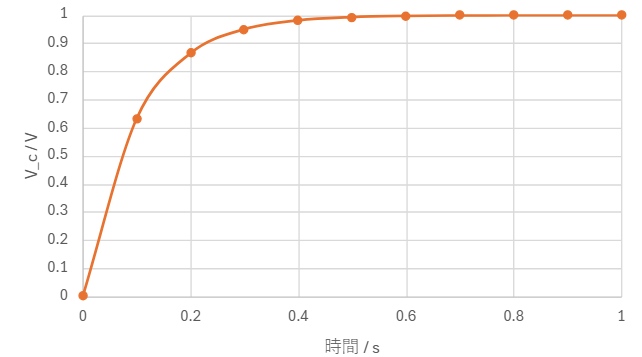
\includegraphics[width=0.7\linewidth]{simg1.png}
    \caption{理論値での$V_c$}
\end{figure}
表と波形より，理論値とシミュレーション値は全体にわたって非常によく一致していることが確認できる。
両者の差はごくわずかであり，数値計算における丸め誤差の範囲内であると考えられる。


\subsection{実験２}
$t=0.83\,\mathrm{s}$を式(2)に代入すると、
\[
V_c(0.83) = 1 - e^{-10\times0.83} = 1-e^{-8.3}= 0.999751\ldots 
\]
となり、収束値である1$V$に十分近い値になっていることが分かる。また、表2から有効数字4桁で評価すると
$t=0.8\,\mathrm{s}$からの$V_c$の変化がほとんど見られなくなり、$t=0.83\,\mathrm{s}$を定常状態の
開始時刻とするのは妥当であると考えられる。

\subsection{実験３}
交流電圧源
\[
V(t)=\sin(\omega t)
\]
を入力したRC回路について,回路方程式は

\[
\sin(\omega t)=RC\frac{dV_c(t)}{dt}+V_c(t)
\]

となる。
初期条件
\[
V_c(0)=0
\]
のもとで両辺をラプラス変換すると，

\[
RC(sV_c(s)-V_c(0))+V_c(s)
=
\frac{\omega}{s^2+\omega^2}
\]

初期条件を代入して整理すると

\[
V_c(s)
=
\frac{\omega}{(s^2+\omega^2)(RCs+1)}
\]

を得る。
これを逆ラプラス変換すると，一般解

\[
V_c(t)
=
Ae^{-t/RC}
+
\frac{1}{\sqrt{1+(\omega RC)^2}}
\sin(\omega t-\phi)
\]

が得られる。ただし

\[
\phi=\tan^{-1}(\omega RC)
\]

である。
ここで初期条件
\[
V_c(0)=0
\]

を用いると

\[
A=
\frac{\sin\phi}{\sqrt{1+(\omega RC)^2}}
\]

となるため，最終的に

\begin{equation}
    V_c(t)
=
\frac{\sin\phi}{\sqrt{1+(\omega RC)^2}}
e^{-t/RC}
+
\frac{1}{\sqrt{1+(\omega RC)^2}}
\sin(\omega t-\phi)
\end{equation}


を得る。

第1項は過渡解、第2項は定常解を表し、
過渡項は指数関数的に減衰するため，
十分時間が経過すると定常解のみが残る。

(3)式に
$R = 10\,\text{k}\Omega,\; C = 10\,\mu\text{F},\; \omega = 2\pi f = 20\pi\,\text{Hz}$
また、これらの数値よりもとめた$\phi$ を代入し、$t = 0 \sim 0.8\,\text{s}$
における$V_{c}$の理論値を算出した。以下に理論値とシミュレーション値をまとめた表を以下に示す。
\begin{table}[H]
\centering
\caption{過渡状態における$V_{c}$の理論値とシミュレーション値の比較}
\begin{tabular}{ccc}
\toprule
時間[s] & 理論値[V] & シミュレーション値[V] \\
\midrule
0.0 & 0.000000 & 0.000000 \\
0.1 & -0.098120 & -0.097972 \\
0.2 & -0.134216 & -0.134113 \\
0.3 & -0.147495 & -0.147362 \\
0.4 & -0.152380 & -0.152210 \\
0.5 & -0.154177 & -0.154066 \\
0.6 & -0.154838 & -0.154702 \\
0.7 & -0.155082 & -0.154911 \\
0.8 & -0.155171 & -0.155059 \\
\bottomrule
\end{tabular}
\end{table}
次に(3)式の定常解のみにtを代入してもとめた理論値とシミュレーション値をまとめた表を以下に示す。
\begin{table}[H]
\centering
\caption{定常状態における$V_{c}$の理論値とシミュレーション値の比較}
\begin{tabular}{ccc}
\toprule
時間[s] & 理論値[V] & シミュレーション値[V] \\
\midrule
0.83 & 0.071462 & 0.071411 \\
0.84 & 0.140099 & 0.140063 \\
0.85 & 0.155223 & 0.155084 \\
0.86 & 0.111057 & 0.111024 \\
0.87 & 0.024471 & 0.024481 \\
0.88 & -0.071462 & -0.071373 \\
0.89 & -0.140099 & -0.139929 \\
0.90 & -0.155223 & -0.155068 \\
0.91 & -0.111057 & -0.110941 \\
0.92 & -0.024471 & -0.024443 \\
0.93 & 0.071462 & 0.071406 \\
\bottomrule
\end{tabular}
\end{table}
表3より、過渡状態における理論値とシミュレーション値は良く一致していることが確認できる。
例えば $t=0.8\,\mathrm{s}$ における差は

\[
|-0.155171-(-0.155059)|
=1.12\times10^{-4}
\]

であり、相対誤差は

\[
\frac{1.12\times10^{-4}}{0.155171}\times100
\simeq 0.072\%
\]

と十分小さい。
したがって、導出した過渡解は
シミュレーション結果を良く再現しているといえる。

また，時間の経過とともに電圧変化が小さくなり、
過渡成分が指数関数的に減衰して定常状態へ移行する様子も確認できた。
これは(3)式第1項で表される過渡解
$Ae^{-t/RC}$
が時間とともに減衰することと対応している。

次に表4より、定常状態においても理論値とシミュレーション値は良く一致した。
例えば $t=0.85\,\mathrm{s}$ における差は

\[
|0.155223-0.155084|
=1.39\times10^{-4}
\]

であり，相対誤差は

\[
\frac{1.39\times10^{-4}}{0.155223}\times100
\simeq0.090\%
\]

である。
誤差は極めて小さく、振幅および位相差を含めて
RC回路の交流定常応答が理論通りであることが確認できた。

さらに、$t=0.83\,\mathrm{s}$と1周期後の
$t=0.93\,\mathrm{s}$で電圧値がほぼ一致していることから、
定常状態における波形の周期性も確認できた。

\subsection{実験４}
(1)式に
$R = 10\,\text{k}\Omega,\; C = 10\,\mu\text{F},\; \omega = 2\pi f = 20\pi\,\text{Hz}$
 を代入し、
各時刻における電流$I$の理論値を算出した。以下に理論値とシミュレーション値をまとめた表を示す。
\begin{table}[H]
\centering
\caption{電流の理論値とシミュレーション値の比較（定常状態）}
\begin{tabular}{ccc}
\toprule
時間[s] & 理論値[A] & シミュレーション値[A] \\
\midrule
0.83 & $8.796 \times 10^{-5}$ & $8.790 \times 10^{-5}$ \\
0.84 & $4.477 \times 10^{-5}$ & $4.477 \times 10^{-5}$ \\
0.85 & $-1.552 \times 10^{-5}$ & $-1.551 \times 10^{-5}$ \\
0.86 & $-6.988 \times 10^{-5}$ & $-6.987 \times 10^{-5}$ \\
0.87 & $-9.755 \times 10^{-5}$ & $-9.749 \times 10^{-5}$ \\
0.88 & $-8.796 \times 10^{-5}$ & $-8.794 \times 10^{-5}$ \\
0.89 & $-4.477 \times 10^{-5}$ & $-4.475 \times 10^{-5}$ \\
0.90 & $1.552 \times 10^{-5}$ & $1.551 \times 10^{-5}$ \\
0.91 & $6.988 \times 10^{-5}$ & $6.984 \times 10^{-5}$ \\
0.92 & $9.755 \times 10^{-5}$ & $9.750 \times 10^{-5}$ \\
0.93 & $8.796 \times 10^{-5}$ & $8.793 \times 10^{-5}$ \\
\bottomrule
\end{tabular}
\end{table}
また、$t = 0.83 \sim 1.2\,\text{s}$
での理論値から得た
電流の波形を以下に示す。
\begin{figure}[H]
    \centering
    \includegraphics[width=0.7\linewidth]{r1.png}
    \caption{理論値での電流の波形}
\end{figure}

一周期後のシミュレーション値にはごくわずかな差が見られるが，
これは数値計算誤差や過渡成分の微小な残存によるものと考えられる。

例えば $t=0.83\,\mathrm{s}$ と $t=0.93\,\mathrm{s}$ の電流値の差は
$3.0\times10^{-8}\,\mathrm{A}$
であり，相対誤差で見ると
\[
\frac{3.0\times10^{-8}}{8.790\times10^{-5}}
\simeq 3.41\times10^{-4}
\]
すなわち$
0.0341\%
$
程度である。
差は極めて小さく，定常状態における波形の周期性を損なうものではないと考えられる。

また，表より理論値とシミュレーション値も非常によく一致していることが分かる。
例えば $t=0.83\,\mathrm{s}$ における相対誤差は
\[
\frac{|8.796-8.790|}{8.796}\times100
\simeq 0.0682\%
\]
であり，非常に小さい。

他の時刻においても同程度の誤差しか見られず，
フェーザ法から得られた理論式がシミュレーション結果と良く一致することが確認できた。

\section{感想}
今回初めてLTspiceを用いたが、回路構成の変更や波形観測が容易であり、
過渡応答や定常応答を視覚的に確認できる点で非常に有用なツールであると感じた。
また、理論式から求めた結果とシミュレーション値を比較することで、RC回路の
振る舞いをより直感的かつ深く理解することができた。

今後は今回使用しなかった機能についても学び，
さまざまな回路解析に活用していきたいと感じた。


















\begin{thebibliography}{99}
    \bibitem{tex}
    LTspiceでグラフの値を正確に読み取る方法（.measコマンド）　\url{https://www.sonohen.page/2022/08/ltspicemeas.html}
\end{thebibliography}


\end{document}
